\documentclass[tikz,border=6pt]{standalone}
\usepackage[T1]{fontenc}
\usepackage{helvet}
\renewcommand{\familydefault}{\sfdefault}
\usetikzlibrary{positioning,arrows.meta,calc,fit,shapes.geometric,shapes.misc,shapes.multipart}
\newcommand{\dt}{\,\textperiodcentered\,}
\tikzset{
  arr/.style={-{Latex[length=2.2mm]},line width=0.6pt},
  darr/.style={{Latex[length=2.2mm]}-{Latex[length=2.2mm]},line width=0.6pt},
  dashedarr/.style={-{Latex[length=2.2mm,open]},line width=0.6pt,dashed},
  retarr/.style={-{Latex[length=2.2mm]},line width=0.6pt,dashed},
  lbl/.style={font=\footnotesize\itshape},
}

\tikzset{
  act/.style={draw,rounded corners=7pt,align=center,font=\small\bfseries,inner sep=7pt,minimum height=1.1cm,minimum width=3.6cm,line width=0.6pt},
  dec/.style={diamond,draw,aspect=2.2,align=center,font=\small\bfseries,inner sep=1pt,line width=0.6pt},
  start/.style={circle,fill=black,minimum size=6mm,inner sep=0pt},
  stop/.style={circle,draw,line width=1pt,minimum size=7mm,inner sep=0pt,path picture={\fill[black] (path picture bounding box.center) circle (2.2mm);}},
  bar/.style={fill=black,minimum height=1.4mm,inner sep=0pt},
  flow/.style={arr},
  g/.style={font=\footnotesize\itshape,fill=white,inner sep=1pt},
}

\begin{document}
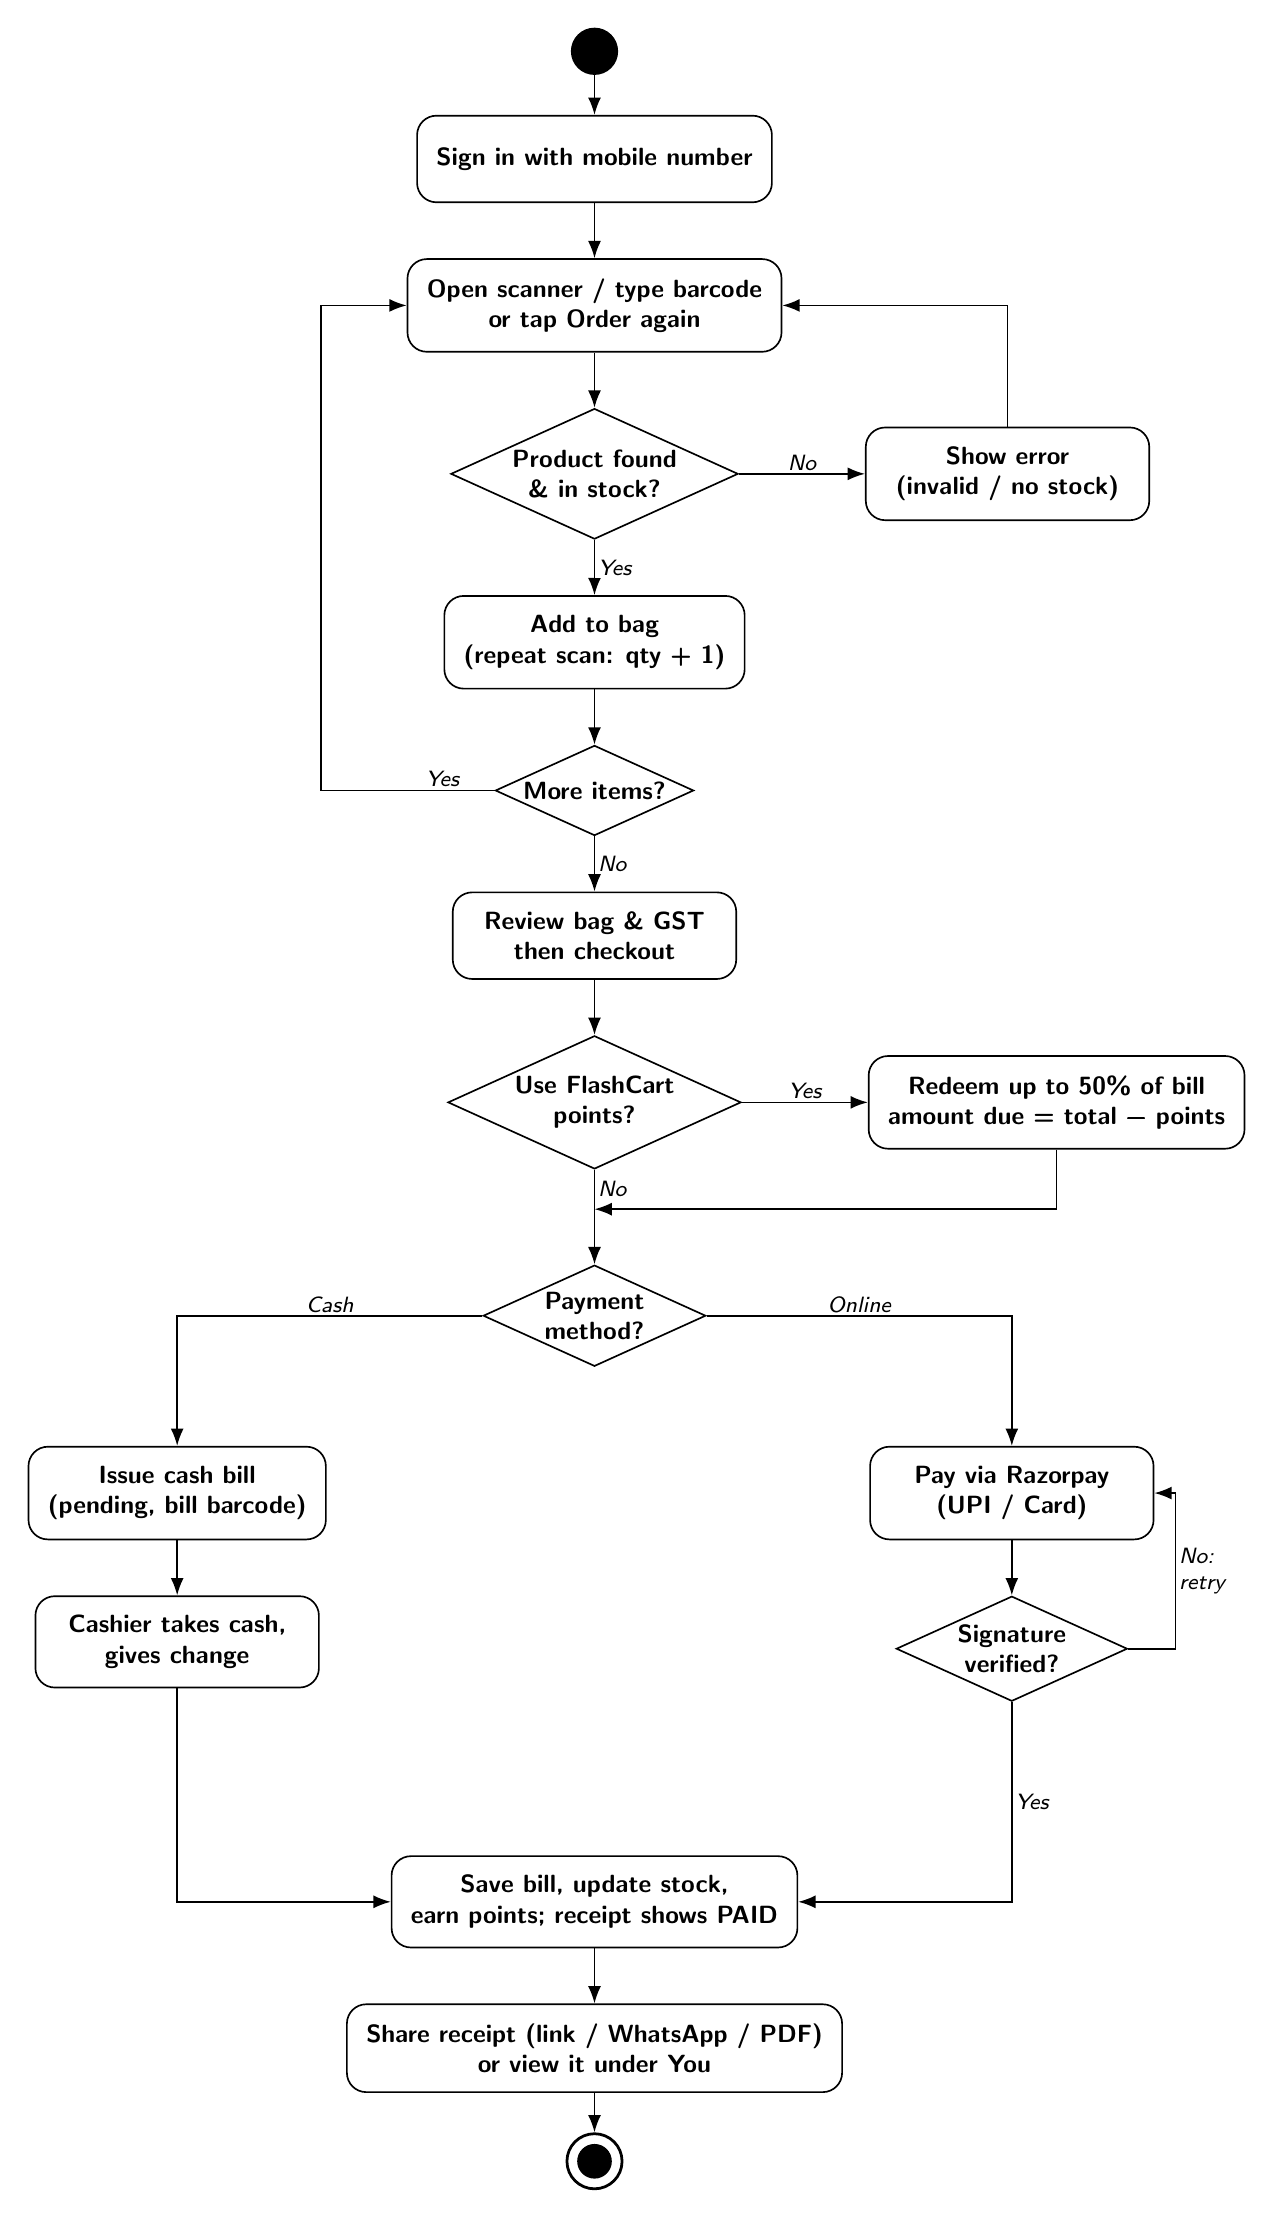
\begin{tikzpicture}[node distance=7mm and 12mm]
\node[start] (s) {};
\node[act,below=5mm of s] (a1) {Sign in with mobile number};
\node[act,below=of a1] (a2) {Open scanner / type barcode\\or tap \emph{Order again}};
\node[dec,below=of a2] (d1) {Product found\\\& in stock?};
\node[act,right=16mm of d1] (err) {Show error\\(invalid / no stock)};
\node[act,below=of d1] (a3) {Add to bag\\(repeat scan: qty + 1)};
\node[dec,below=of a3] (d2) {More items?};
\node[act,below=of d2] (a4) {Review bag \& GST\\then checkout};
\node[dec,below=of a4] (d3) {Use FlashCart\\points?};
\node[act,right=16mm of d3] (a5) {Redeem up to 50\% of bill\\amount due = total \textminus\ points};
\node[dec,below=12mm of d3] (d4) {Payment\\method?};
\node[act,below=10mm of d4,xshift=-5.3cm] (c1) {Issue cash bill\\(pending, bill barcode)};
\node[act,below=of c1] (c2) {Cashier takes cash,\\gives change};
\node[act,below=10mm of d4,xshift=5.3cm] (o1) {Pay via Razorpay\\(UPI / Card)};
\node[dec,below=of o1] (d5) {Signature\\verified?};
\node[act,below=62mm of d4] (a6) {Save bill, update stock,\\earn points; receipt shows PAID};
\node[act,below=of a6] (a7) {Share receipt (link / WhatsApp / PDF)\\or view it under \emph{You}};
\node[stop,below=5mm of a7] (e) {};
\draw[flow] (s) -- (a1);
\draw[flow] (a1) -- (a2);
\draw[flow] (a2) -- (d1);
\draw[flow] (d1) -- node[g,above]{No} (err);
\draw[flow] (err.north) |- ($(a2.east)+(0,0)$);
\draw[flow] (d1) -- node[g,right]{Yes} (a3);
\draw[flow] (a3) -- (d2);
\draw[flow] (d2.west) -- node[g,above,pos=0.3]{Yes} ++(-2.2,0) |- (a2.west);
\draw[flow] (d2) -- node[g,right]{No} (a4);
\draw[flow] (a4) -- (d3);
\draw[flow] (d3) -- node[g,above]{Yes} (a5);
\draw[flow] (a5.south) |- ($(d3.south)+(0,-5mm)$);
\draw[flow] (d3) -- node[g,right,pos=0.2]{No} (d4);
\draw[flow] (d4.west) -| node[g,above,pos=0.25]{Cash} (c1.north);
\draw[flow] (c1) -- (c2);
\draw[flow] (c2.south) |- (a6.west);
\draw[flow] (d4.east) -| node[g,above,pos=0.25]{Online} (o1.north);
\draw[flow] (o1) -- (d5);
\draw[flow] (d5.east) -- ++(0.6,0) |- node[g,right,pos=0.25,align=left]{No:\\retry} (o1.east);
\draw[flow] (d5.south) |- node[g,right,pos=0.25]{Yes} (a6.east);
\draw[flow] (a6) -- (a7);
\draw[flow] (a7) -- (e);
\end{tikzpicture}
\end{document}
